% Options for packages loaded elsewhere
\PassOptionsToPackage{unicode}{hyperref}
\PassOptionsToPackage{hyphens}{url}
\PassOptionsToPackage{dvipsnames,svgnames,x11names}{xcolor}
%
\documentclass[
  letterpaper,
  DIV=11,
  numbers=noendperiod]{scrartcl}

\usepackage{amsmath,amssymb}
\usepackage{lmodern}
\usepackage{iftex}
\ifPDFTeX
  \usepackage[T1]{fontenc}
  \usepackage[utf8]{inputenc}
  \usepackage{textcomp} % provide euro and other symbols
\else % if luatex or xetex
  \usepackage{unicode-math}
  \defaultfontfeatures{Scale=MatchLowercase}
  \defaultfontfeatures[\rmfamily]{Ligatures=TeX,Scale=1}
\fi
% Use upquote if available, for straight quotes in verbatim environments
\IfFileExists{upquote.sty}{\usepackage{upquote}}{}
\IfFileExists{microtype.sty}{% use microtype if available
  \usepackage[]{microtype}
  \UseMicrotypeSet[protrusion]{basicmath} % disable protrusion for tt fonts
}{}
\makeatletter
\@ifundefined{KOMAClassName}{% if non-KOMA class
  \IfFileExists{parskip.sty}{%
    \usepackage{parskip}
  }{% else
    \setlength{\parindent}{0pt}
    \setlength{\parskip}{6pt plus 2pt minus 1pt}}
}{% if KOMA class
  \KOMAoptions{parskip=half}}
\makeatother
\usepackage{xcolor}
\setlength{\emergencystretch}{3em} % prevent overfull lines
\setcounter{secnumdepth}{-\maxdimen} % remove section numbering
% Make \paragraph and \subparagraph free-standing
\ifx\paragraph\undefined\else
  \let\oldparagraph\paragraph
  \renewcommand{\paragraph}[1]{\oldparagraph{#1}\mbox{}}
\fi
\ifx\subparagraph\undefined\else
  \let\oldsubparagraph\subparagraph
  \renewcommand{\subparagraph}[1]{\oldsubparagraph{#1}\mbox{}}
\fi


\providecommand{\tightlist}{%
  \setlength{\itemsep}{0pt}\setlength{\parskip}{0pt}}\usepackage{longtable,booktabs,array}
\usepackage{calc} % for calculating minipage widths
% Correct order of tables after \paragraph or \subparagraph
\usepackage{etoolbox}
\makeatletter
\patchcmd\longtable{\par}{\if@noskipsec\mbox{}\fi\par}{}{}
\makeatother
% Allow footnotes in longtable head/foot
\IfFileExists{footnotehyper.sty}{\usepackage{footnotehyper}}{\usepackage{footnote}}
\makesavenoteenv{longtable}
\usepackage{graphicx}
\makeatletter
\def\maxwidth{\ifdim\Gin@nat@width>\linewidth\linewidth\else\Gin@nat@width\fi}
\def\maxheight{\ifdim\Gin@nat@height>\textheight\textheight\else\Gin@nat@height\fi}
\makeatother
% Scale images if necessary, so that they will not overflow the page
% margins by default, and it is still possible to overwrite the defaults
% using explicit options in \includegraphics[width, height, ...]{}
\setkeys{Gin}{width=\maxwidth,height=\maxheight,keepaspectratio}
% Set default figure placement to htbp
\makeatletter
\def\fps@figure{htbp}
\makeatother

\KOMAoption{captions}{tableheading}
\makeatletter
\makeatother
\makeatletter
\makeatother
\makeatletter
\@ifpackageloaded{caption}{}{\usepackage{caption}}
\AtBeginDocument{%
\ifdefined\contentsname
  \renewcommand*\contentsname{Table of contents}
\else
  \newcommand\contentsname{Table of contents}
\fi
\ifdefined\listfigurename
  \renewcommand*\listfigurename{List of Figures}
\else
  \newcommand\listfigurename{List of Figures}
\fi
\ifdefined\listtablename
  \renewcommand*\listtablename{List of Tables}
\else
  \newcommand\listtablename{List of Tables}
\fi
\ifdefined\figurename
  \renewcommand*\figurename{Figure}
\else
  \newcommand\figurename{Figure}
\fi
\ifdefined\tablename
  \renewcommand*\tablename{Table}
\else
  \newcommand\tablename{Table}
\fi
}
\@ifpackageloaded{float}{}{\usepackage{float}}
\floatstyle{ruled}
\@ifundefined{c@chapter}{\newfloat{codelisting}{h}{lop}}{\newfloat{codelisting}{h}{lop}[chapter]}
\floatname{codelisting}{Listing}
\newcommand*\listoflistings{\listof{codelisting}{List of Listings}}
\makeatother
\makeatletter
\@ifpackageloaded{caption}{}{\usepackage{caption}}
\@ifpackageloaded{subcaption}{}{\usepackage{subcaption}}
\makeatother
\makeatletter
\@ifpackageloaded{tcolorbox}{}{\usepackage[many]{tcolorbox}}
\makeatother
\makeatletter
\@ifundefined{shadecolor}{\definecolor{shadecolor}{rgb}{.97, .97, .97}}
\makeatother
\makeatletter
\makeatother
\ifLuaTeX
  \usepackage{selnolig}  % disable illegal ligatures
\fi
\IfFileExists{bookmark.sty}{\usepackage{bookmark}}{\usepackage{hyperref}}
\IfFileExists{xurl.sty}{\usepackage{xurl}}{} % add URL line breaks if available
\urlstyle{same} % disable monospaced font for URLs
\hypersetup{
  pdftitle={DS4I Project 2},
  colorlinks=true,
  linkcolor={blue},
  filecolor={Maroon},
  citecolor={Blue},
  urlcolor={Blue},
  pdfcreator={LaTeX via pandoc}}

\title{DS4I Project 2}
\author{}
\date{}

\begin{document}
\maketitle
\ifdefined\Shaded\renewenvironment{Shaded}{\begin{tcolorbox}[borderline west={3pt}{0pt}{shadecolor}, frame hidden, breakable, interior hidden, enhanced, sharp corners, boxrule=0pt]}{\end{tcolorbox}}\fi

\renewcommand*\contentsname{Table of contents}
{
\hypersetup{linkcolor=}
\setcounter{tocdepth}{3}
\tableofcontents
}
\hypertarget{abstract}{%
\subsection{Abstract}\label{abstract}}

\hypertarget{introduction}{%
\subsection{Introduction}\label{introduction}}

A State of Nation Address (SONA) is a speech given by the President of
South Africa in which the president reports on the status of the nation.
It functions as an annual report that include political and
socio-economic topics. These include but not limited to topics
surrounding the nation's budget, economy, news, agenda, progress,
achievements and the president's priorities and legislative proposals.
The SONA gives us an idea of broader political landscape and
socio-economic issues and challenges that are plauging the country. At
the same time, it also reflect on the achievements and growth and
progress the country has made in the past year. Furthermore, it provides
us with a direction and understanding of the countries plans. With that
being said, to comprehensively analyze the history of the SONA speeches
will provide us extensive perspective and viewpoint of the struggles and
triumph over the course of South Africa.

In this assignment, we aim to provide that perspective and viewpoint
from a computational approach. We will utilize sentiment analysis and
topic modelling techniques to quantified the emotional tone of each
president and reoccurring topics that will provide context and
understanding to the broader socio-political and economic environment of
South Africa. More specifically, utilizing sentiment analysis and a
topic modelling technique called Latent Dirichlet Allocation (LDA) to
analyze the SONA speeches from 1994 and 2022.

Sentiment analysis refers to the use of natural language processing
(NLP), text analysis, computational linguistics, to identify, extract,
quantify, and study affective states and subjective information.
Furthermore, Topic modelling is a statistical and unsupervised learning
technique to identify and discover topics within a collection of text or
documents. It is commonly used to classify documents and discover hidden
semantic properties in a corpus of text.

A related study involves exploring sentiment and topics from Philippine
President in the SONA from John Miranda and Rex P. Bringula (2021). The
study showcased the SONAs generally expressed positive sentiments while
the lowest negative sentiment was during the martial law period in 1974
Furthermore, another related study includes Mining Tourist's Perception
toward Indonesia Tourism Destination. Results shows that Joy is the most
prominent emotion accompanying visitors' experiences (Herry Irawan,
Riefvan Achmad (2019)).

The relevant work showcases that researchers have found significant
results when investigating documents of texts with regards to evaluating
emotive content or extracting common themes and topics.

\hypertarget{sentiment-analysis}{%
\subsection{Sentiment Analysis}\label{sentiment-analysis}}

\hypertarget{topic-modelling}{%
\subsection{Topic Modelling}\label{topic-modelling}}

\hypertarget{trends}{%
\subsection{Trends}\label{trends}}

In this study, we embarked on descriptive analysis of the content of the
State of\\
Nations Address speeches by South African presidents from 1994 to 2022.
We uti-\\
lizing advanced sentiment analysis, and topic modelling techniques to
quantified\\
the emotional tone of each speech and general topics that will provide
context and\\
understanding to the broader socio-political environment of South Africa
over time.\\
We utilized the Afinn lexicon which is a list of English terms manually
rated for\\
valence with an integer between -5 (negative) and +5 (positive).

\hypertarget{yearly-trends}{%
\subsubsection{Yearly Trends}\label{yearly-trends}}

Figure 1 displays the average sentiment segregated by year and
president. Nelson\\
Mandela's term, symbolizing the dawn of democracy in South Africa
manifested\\
positive sentiment scores. However, there is a sharp decline after that
from 1995-\\
1999. Furthermore, we notice that Mbeki in the early 2000's had more
positive\\
sentiment as compared to the late 90's. However, this sentiment
diminishes over\\
his tenure, possibly indicating challenges or controversial issues faced
during his\\
presidency. Zuma's term showcases dramatic peaks and valleys in
sentiment scores.\\
We notice a steady increase in positive sentiment in the late 2000's
peaking in 2010\\
at a sentiment score of 1.25. Various factors could be investigated for
this. A possible\\
reason for this is the 2010 FIFA World Cup that was hosted in South
Africa.\\
However, after the world cup (2010) we notice a volatile pattern
associated with\\
Zuma's tenure as contrast to the high witnessed in 2010, there was a
drop leading\\
to a sentiment score of below 0.5 in 2013.\\
Furthermore, ever since Ramaphosa has been elected into office in 2018,
we notice\\
a steady decline in sentiment score. A possible reason for this could be
the load-\\
shedding and Coronavirus struggles that have plagued our country in
recent years.\\
These will be further investigated in the section.

\begin{figure}

{\centering \includegraphics{docs/Sent_trend_year.pdf}

}

\caption{Yearly Sentiment Trends segregated by presidents.}

\end{figure}

Figure 2 echos the analysis that is portrayed in Figure 1. A further
comment can\\
be extremely negative or positive sentiments (-5 and 5) are sparsely
represented\\
across the years, indicating that highly polarized sentiments are rare
in the dataset.\\
Throughout most of the years, the neutral sentiment (values 1 and 2)
remains pre-\\
dominant, suggesting a generally stable mood or balanced content in the
analyzed\\
texts.

\begin{figure}

{\centering 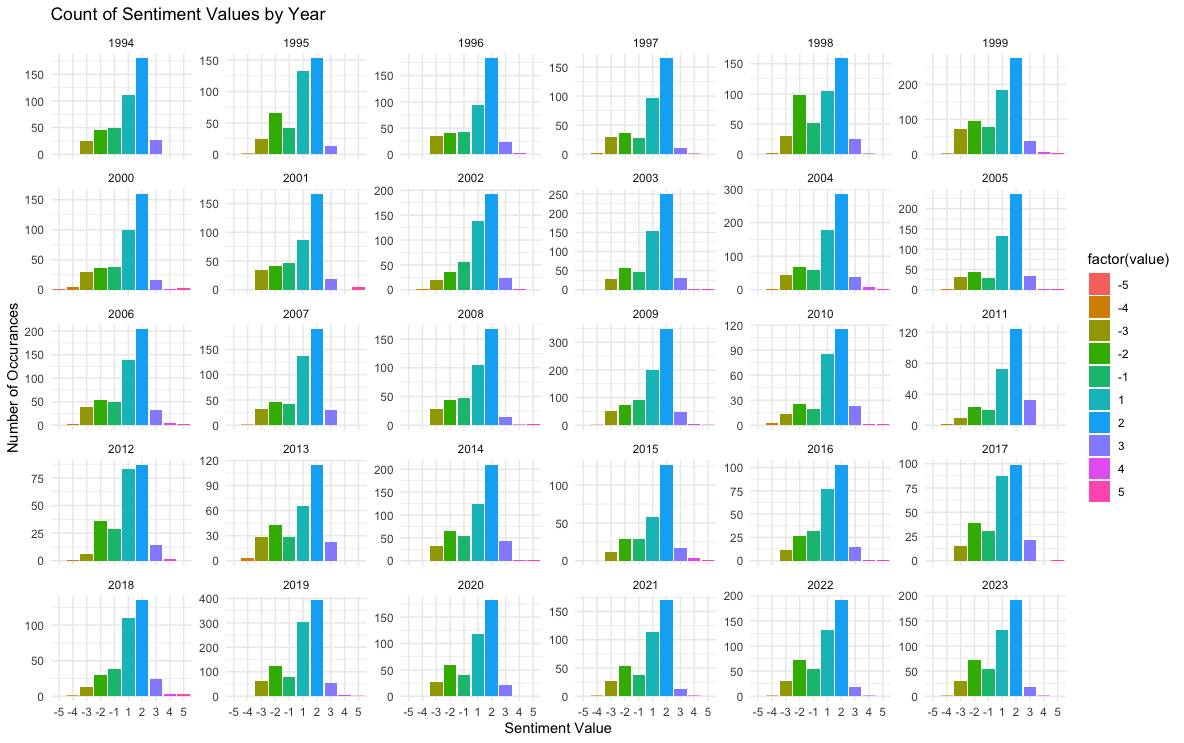
\includegraphics{docs/Count_Sentiment_Values_by_Year.png}

}

\caption{Sentiment Valence Trends by year}

\end{figure}

\hypertarget{decade-trends}{%
\subsubsection{Decade Trends}\label{decade-trends}}

Within the span of three decades, Figure 3 illustrates the average
sentiment per\\
decade. The 2000s and 2010s emerge as periods marked by heightened
positive\\
sentiment. In contrast, the 1990s and the 2020s manifest a more tempered
positivity.\\

\begin{figure}

{\centering 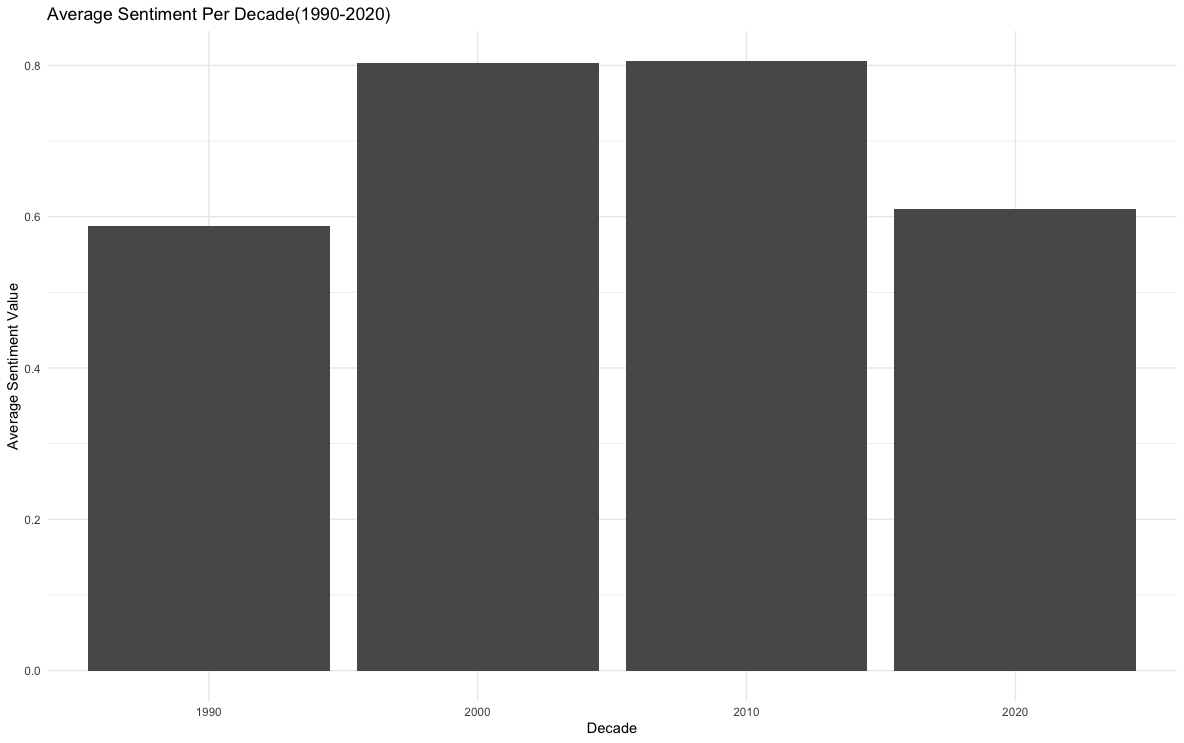
\includegraphics{docs/Per_Decade.png}

}

\caption{Average Sentiment Score Per Decade}

\end{figure}

\hypertarget{pre-and-post-election-trends}{%
\subsubsection{Pre and Post Election
Trends}\label{pre-and-post-election-trends}}

Figure 4 depicts the average sentiment during the pre and post-election
phases for\\
several South African presidents, namely Mandela, Mbeki, Ramaphosa, and
Zuma.\\
Analyzing the sentiment before the elections (pre) for each president
reveals a trend.\\
Generally, the sentiment before the election is comparatively more
negative or less\\
positive than the post-election phase. This pattern could be attributed
to the strategic communication employed during election campaigns. It's
common during election campaigns for leaders or political parties to
highlight existing problems or crises to win voter trust by promising
solutions. By making the situation seem more critical, candidates can
position themselves as the needed change.

\begin{figure}

{\centering 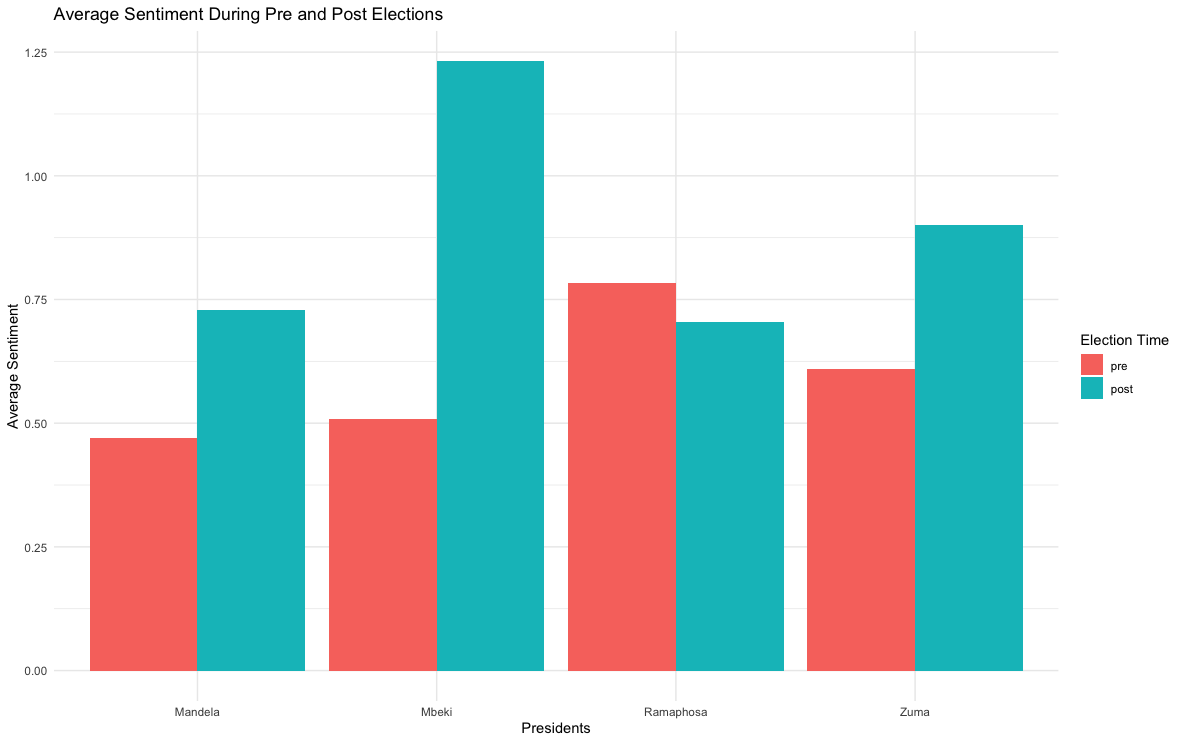
\includegraphics{docs/Pre_post_elections.png}

}

\caption{Comparing average sentiment scores pre and post elections.}

\end{figure}

\hypertarget{topic-modelling-trends}{%
\subsection{Topic Modelling Trends}\label{topic-modelling-trends}}

\begin{figure}

{\centering 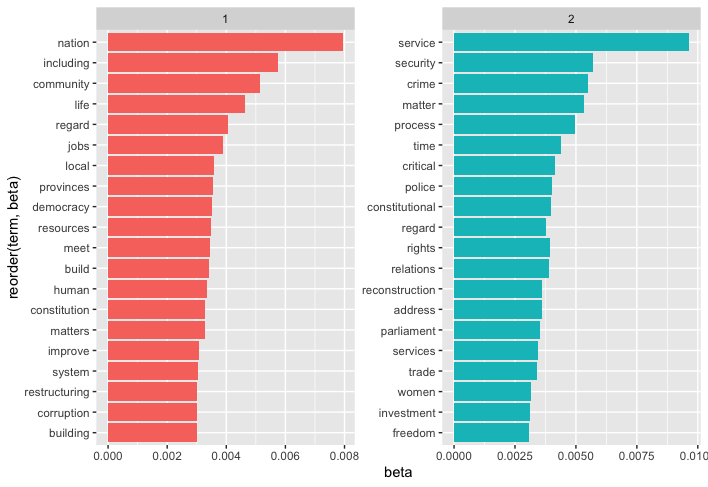
\includegraphics{docs/lda_1990.pdf}

}

\caption{Figure demonstrating two topics against beta from 1994-1999}

\end{figure}

\begin{figure}

{\centering 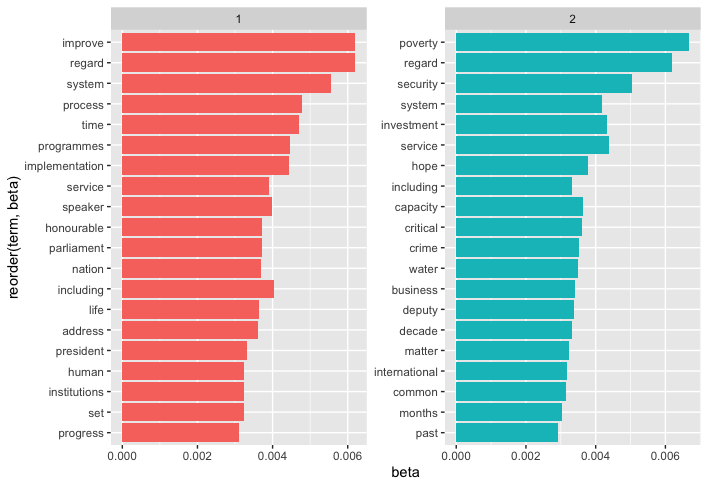
\includegraphics{docs/lda_2000.pdf}

}

\caption{Figure demonstrating two topics against beta from 2000-2010}

\end{figure}

\begin{figure}

{\centering 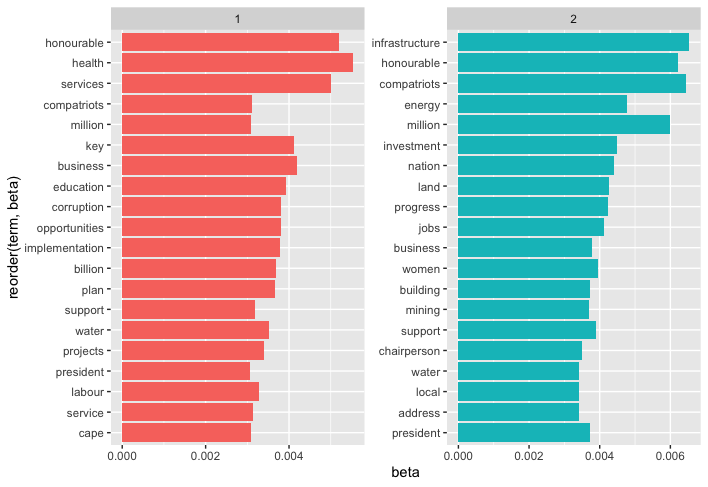
\includegraphics{docs/lda_2010.pdf}

}

\caption{Figure demonstrating two topics against beta from 2010-2020}

\end{figure}

\begin{figure}

{\centering 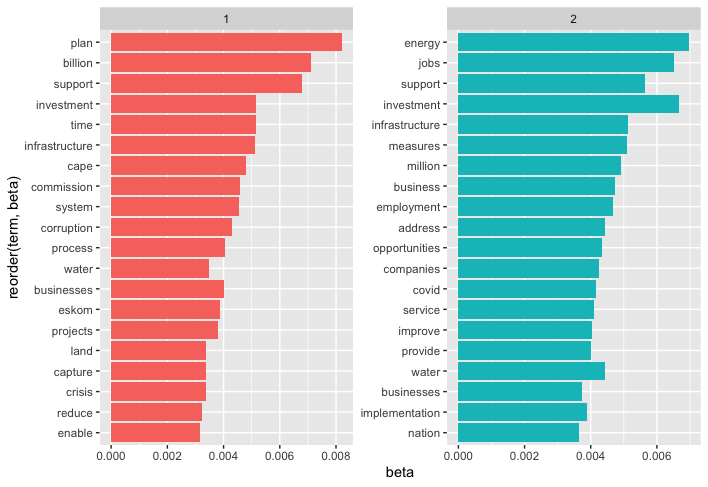
\includegraphics{docs/lda_2020.pdf}

}

\caption{Figure demonstrating two topics against beta from 2020-2022}

\end{figure}

\hypertarget{overall-trends}{%
\subsubsection{Overall Trends}\label{overall-trends}}

It is found that the SONA's generally expressed positive sentiments
post-elections,\\
as supposed to pre-elections. Another finding, indicated a more negative
sentiment\\
in the speeches during the 1990s and the 2020s when juxtaposed against
the relatively more positive undertones from 2000 to 2020. These
sentiment shifts keenly reflect the changing political landscape and
challenges faced in South Africa during these periods. Overall, our
findings reveal distinct shifts in the emotional undertones of
presidential speeches over time, providing insights into the evolving
political narratives and concerns of the nation.

\hypertarget{discussion}{%
\subsection{Discussion}\label{discussion}}



\end{document}
